\documentclass[twocolumn,twoside,11pt,a4paper]{article}
%----------------------------------------------------------------------------------------
%	packages
%----------------------------------------------------------------------------------------

\usepackage[english]{babel}  % portuguese
\usepackage{graphicx}           % images: .png or .pdf w/ pdflatex; .eps w/ latex
\usepackage{lipsum}             % generate dummy text throughout this template

%% For iso-8859-1 (latin1), comment next line and uncomment the second line
\usepackage[utf8]{inputenc}
%\usepackage[latin1]{inputenc}

\usepackage[T1]{fontenc}        % T1 fonts
\usepackage{lmodern}            % fonts
\usepackage[sc]{mathpazo}       % Use the Palatino font
\linespread{1.05}               % Line spacing - Palatino needs more space between lines
\usepackage{microtype}          % Slightly tweak font spacing for aesthetics
\usepackage{url}                % urls
\usepackage[hang, small, labelfont=bf,up,textfont=it,up]{caption} % Custom captions under/above floats in tables or figures
\usepackage{booktabs}           % Horizontal rules in tables
\usepackage{float}              % Required for tables and figures in the multi-column environment - they need to be placed in specific locations with the [H] (e.g. \begin{table}[H])
\usepackage{paralist}           % Used for the compactitem environment which makes bullet points with less space between them
\usepackage{pdfpages}

% geometry package
\usepackage[outer=20mm,inner=20mm,vmargin=15mm,includehead,includefoot,headheight=15pt]{geometry}
%% space between columns
\columnsep 10mm

\usepackage{abstract}           % Allows abstract customization
\renewcommand{\abstractnamefont}{\normalfont\bfseries} % Set the "Abstract" text to bold
\renewcommand{\abstracttextfont}{\normalfont\small\itshape} % Set the abstract itself to small italic text

% \usepackage{titlesec}           % Allows customization of titles
% \renewcommand\thesection{\Roman{section}} % Roman numerals for the sections
% \renewcommand\thesubsection{\Roman{subsection}} % Roman numerals for subsections
% \titleformat{\section}[block]{\large\scshape\centering}{\thesection.}{1em}{} % Change the look of the section titles
% \titleformat{\subsection}[block]{\large}{\thesubsection.}{1em}{} % Change the look of the section titles

\usepackage[pdftex]{hyperref}
\hypersetup{%
    a4paper = true,              % use A4 paper 
    bookmarks = true,            % make bookmarks 
    colorlinks = true,           % false: boxed links; true: colored links
    pdffitwindow = false,        % page fit to window when opened
    pdfpagemode = UseNone,       % do not show bookmarks
    pdfpagelayout = SinglePage,  % displays a single page
    pdfpagetransition = Replace, % page transition
    linkcolor=blue,              % hyperlink colors
    urlcolor=blue,
    citecolor=blue,
    anchorcolor=green
}

\usepackage{indentfirst}         % indent also 1st paragraph

\usepackage{fancyhdr}            % Headers and footers
\pagestyle{fancy}                % pages have headers and footers
\fancyhead{}                     % Blank out the default header
\fancyfoot{}                     % Blank out the default footer
\fancyhead[LO,RE]{Exemplo de artigo em \LaTeX} % Custom header text
\fancyhead[RO,LE]{\thepage}      % Custom header text
\fancyfoot[RO,LE]{Grupo xx, \today} % Custom footer text
\renewcommand{\headrulewidth}{0.4pt}
\renewcommand{\footrulewidth}{0.4pt}

%\hyphenation{}                  % explicit hyphenation

%----------------------------------------------------------------------------------------
%	macro definitions
%----------------------------------------------------------------------------------------

% entities
\newcommand{\class}[1]{{\normalfont\slshape #1\/}}
\newcommand{\svg}{\class{SVG}}
\newcommand{\scada}{\class{SCADA}}
\newcommand{\scadadms}{\class{SCADA/DMS}}

%----------------------------------------------------------------------------------------
%	TITLE SECTION
%----------------------------------------------------------------------------------------

\title{\vspace{-15mm}\fontsize{24pt}{10pt}\selectfont\textbf{BOOK PROJ}} % Article title

\author{Afonso Mendonça\\
\small \texttt{up201706708@fe.up.pt}\\
\and
Joaquim Rodrigues\\
\small \texttt{up201704844@fe.up.pt}
\vspace{-5mm}
\and
Joel Coelho\\
\small \texttt{up201909577@fe.up.pt}
\vspace{-5mm}
\and
Pasit Khantigul\\
\small \texttt{up202010272@edu.fe.up.pt}
\vspace{-5mm}
}

\date{\today}

%----------------------------------------------------------------------------------------

\begin{document}

\maketitle
\thispagestyle{plain}            % no headers in the first page

%----------------------------------------------------------------------------------------
%	ABSTRACT
%----------------------------------------------------------------------------------------

\begin{abstract}

The proposed project, \textbf{MUSIC PROJ}, is a full-stack application capable of displaying book-related information. It is divided into two components: backend and user interface. The backend will be responsible for gathering literature information from DBpedia’s API that will be shown according to the user’s search. The user interface will arrange this information in a visually appealing way inciting the user to explore and learn more about their favorite books, authors and subjects. 

\end{abstract}

%----------------------------------------------------------------------------------------
%	ARTICLE CONTENTS
%----------------------------------------------------------------------------------------

\section{Introduction}\label{sec:intro}

This article intends to give more insight into the project the team proposed to do for the Markup Languages and Document Processing curricular unit. We are going to approach the proposal, state of the art, data sources and models and we’ll also give some insight on the development scheduling.

%------------------------------------------------

\section{Proposal}\label{sec:proposal}

The project proposal is based on an application capable of gathering information and being able to display it in an organized and user-friendly manner, allowing the user to explore several book-related fields like author, genre, subject, publisher, etc. The exploring sentiment is specially important to the project and the user experience. With this being said, we can divide our project into two main components.

\subsection{User interface} \label{userinterface} 

The user interface will consist of two main elements: the search-box, where the user can input text that will be used to make queries either for books, authors, publishers or subjects; the node view, where the query result will be displayed as a node and root of a tree. From this point on, the user can interact  with the the nodes either by seeing more information about it, reading the abstract and number of pages of a book for example, or by expanding it and showing its children. This way the user can easily query for an author, for example, select any book written by the author and then select the subject, expanding the node and see other books with the same subject.
By arranging the information as nodes with edges to related works, authors, subjects, etc, we are hoping to create a very pleasant experience where exploration is rewarded and the user can, hopefully, easily find books, authors and subjects that interest them.

\subsection{Backend} \label{backend} 

Responsible for the connection to DBpedia’s API and subsequent queries to fetch user-required information \cite{dbpedia}. It will filter the fields and available entities so that the information retrieved to the user is the most relevant possible. This is specially important since every entity can have a lot of types, different fields and information. Having a quality criteria in terms of what entity types and fields we will accept and display is import so that we can keep information as consistent, meaningful and overall of highest quality as possible since there are some fields that don't exist in, for example, every "book" type entity nor does every "book" type entity also has the same number of other entity types.

%------------------------------------------------

\section{Data sources and models}\label{sec:data}

The data will be provided by DBpedia, as expected. The user will start by filling the search field to create a query whose result will be filtered according to the available entity types. The several fields related to the query result will be displayed, where some are static, giving plain information, and others can link to other entities of the types below. By expanding those relationships, the user can then explore different subjects, authors, books, publishers, etc.

\begin{dataFigure}
    \centering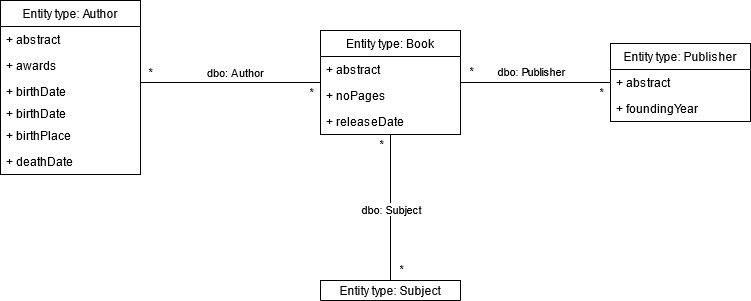
\includegraphics[width=1.0\linewidth]{dataModel.jpg}
    \captionof{figure}{Data model}
\end{dataFigure}

These are the entity types we found out to be consistent and relevant, but these may change during development. There are other many other fields and relationships to entities that are relevant but turn out to be inconsistent, not existing in, for example, every book, like mentioned before. In the other hand, there's a lot of fields and relationships that are consistent but aren't relevant to the user experience.

%------------------------------------------------

\section{State of the Art}\label{sec:conclusions}

 In an era of growing applications, those related to books aren’t an exception \cite{bookApps}. As a result of this, there are apps that are well established on this market such as  \textbf{Amazon kindle}, \textbf{Goodreads} and \textbf{Blinkist}. They share the same key features: allow a user to get to know more about books. Besides allowing the user to explore, search, read and get to know more about a book’s information such as its abstract, author, etc., each app features a unique feature.

\begin{itemize}
    \item Amazon Kindle - Page flip, as it mimics the sensation of reading a book instead of a screen \cite{amazonKindle}
    \item Goodreads - Barcode scanner that allows adding paper books to a “to read” list \cite{goodreads}
    \item Blinklist - Allows the user to switch between audio and read mode. \cite{blinklist}
\end{itemize}

%------------------------------------------------

\section{Schedule}\label{sec:conclusions}

The schedule is reflected in the Gantt chart below.

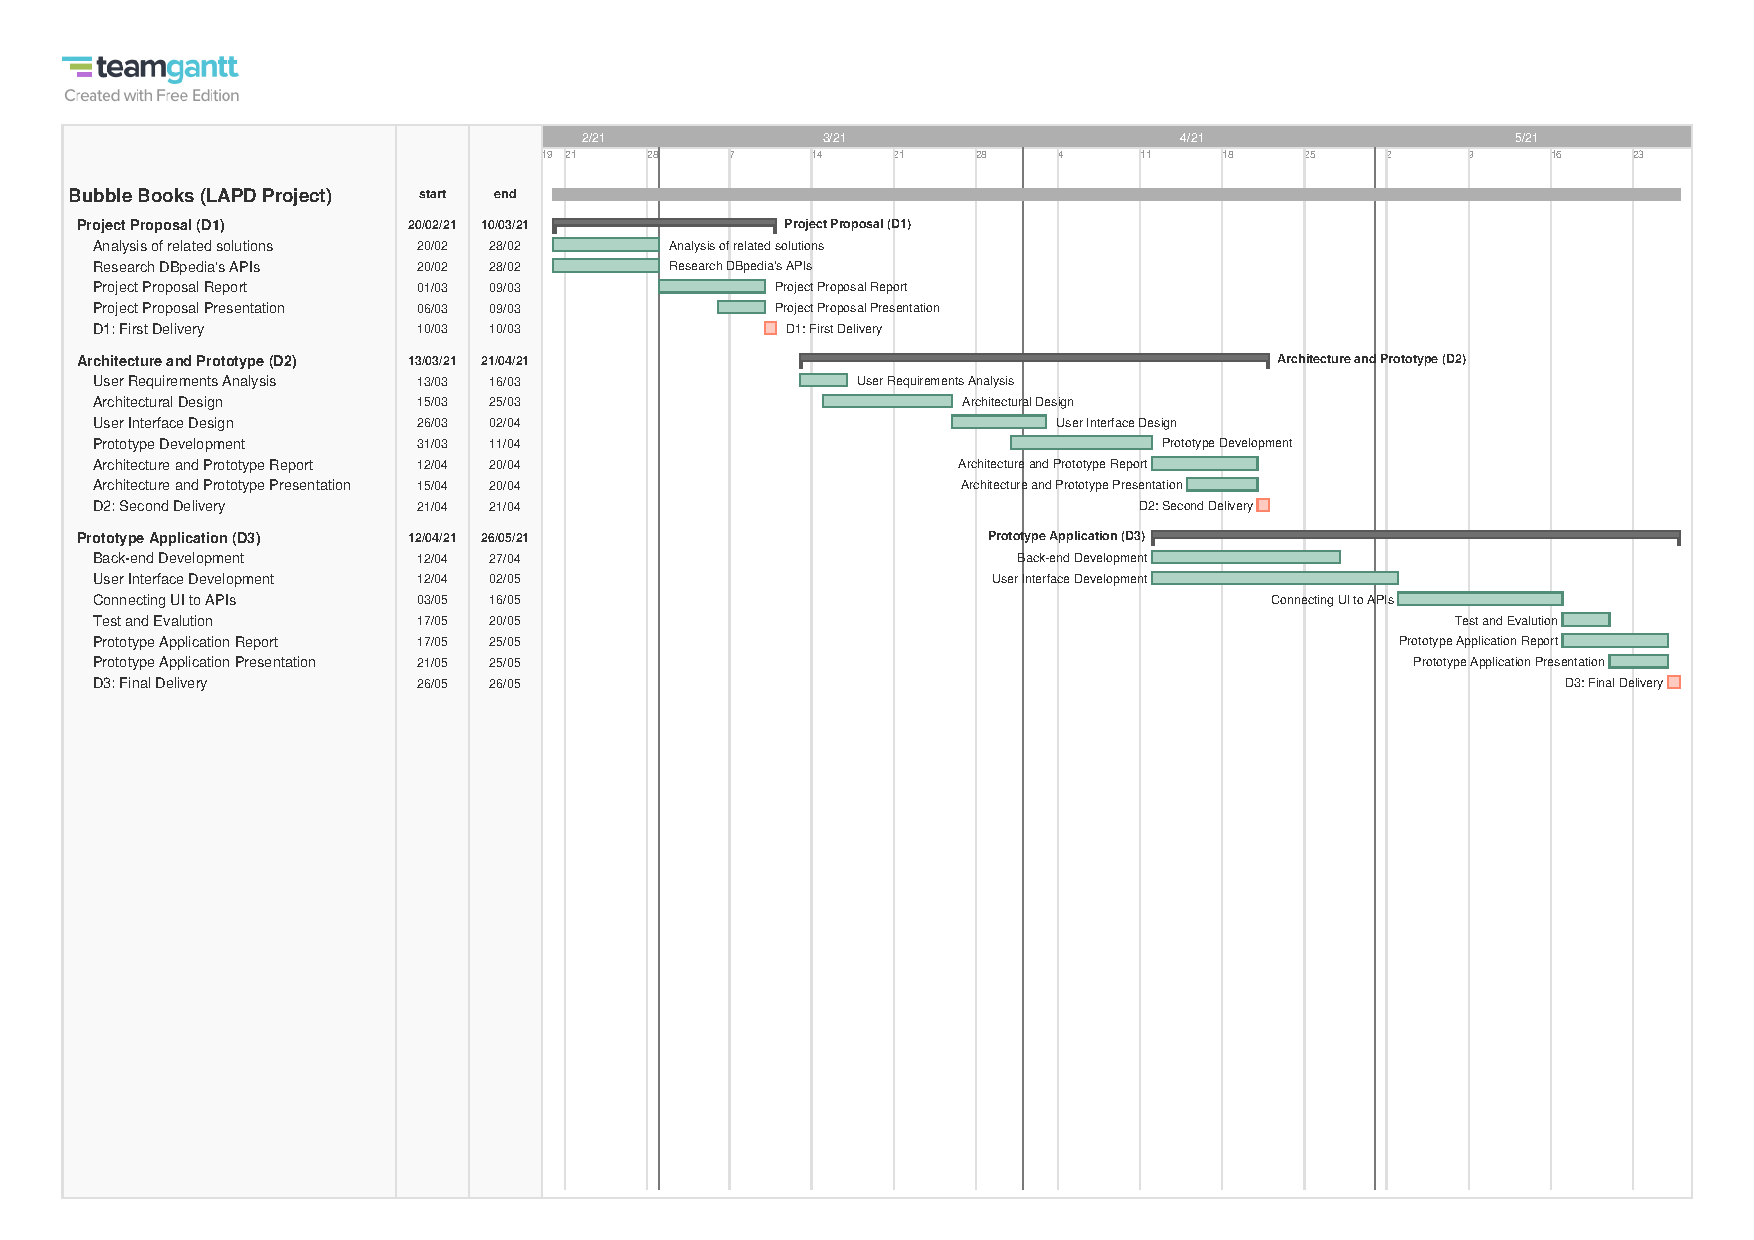
\includepdf[pages=-]{gantt.pdf}


%------------------------------------------------

\section{Conclusions}\label{sec:conclusions}

The team is excited to start the development of project. From the challenge of doing something so visual and focused on the user experience to the actual practical use of the project, there are many factors that make this project very interesting and the team is eager to start working.


%----------------------------------------------------------------------------------------
%	REFERENCE LIST
%----------------------------------------------------------------------------------------
\begin{thebibliography}{9}
\bibitem{dbpedia} 
DBpedia 
\url{https://wiki.dbpedia.org/OnlineAccess#1.4\%20REST\%20API}. 
Last visited on March 2021


\bibitem{bookApps} 
Apps for books
\url{https://www.intellectsoft.net/blog/best-apps-for-book-lovers/}. 
Last visited on March 2021


\bibitem{amazonKindle} 
Amazon Kindle
\url{https://www.amazon.com/kindle-dbs/fd/kcp/ref=klp_mn}. 
Last visited on March 2021


\bibitem{goodreads} 
Goodreads 
\url{https://www.goodreads.com/}. 
Last visited on March 2021


\bibitem{blinklist} 
Blinklist
\url{https://www.blinkist.com/}. 
Last visited on March 2021

\end{thebibliography}

%% auto bibliographic list 
\renewcommand{\bibname}{Referências}
% uses bibtex file
%\bibliographystyle{alpha-pt}
%\bibliographystyle{alpha}
\bibliographystyle{unsrt-pt}
%\bibliographystyle{unsrt}
\bibliography{artigo}

%----------------------------------------------------------------------------------------

\end{document}


